\section{函数项级数的一致收敛性,一致收敛级数的基本性质}

\subsection{函数项级数的一致收敛性}
我们知道,有限个连续函数的和仍然是连续函数,
有限个函数的和的导数及积分也分别等于它们的导数及积分的和.
但是对于无穷多个函数的和是否也具有这些性质呢?
换句话说,无穷多个连续函数的和\(s(x)\)是否仍然是连续函数?
无穷多个函数的导数及积分的和是否仍然分别等于它们的和函数的导数及积分呢?
我们曾经指出,对于幂级数来说,答案是肯定的.
但是对于一般的函数项级数是否都是如此呢?下面来看一个例子.
\begin{example}
函数项级数\[
x + (x^2-x) + (x^3-x^2) + \dotsb + (x^n-x^{n-1}) + \dotsb
\]的每一项都在\([0,1]\)上连续,其前\(n\)项之和为\[
s_n(x) = x^n,
\]因此和函数为\[
s(x) = \lim_{n\to\infty} s_n(x)
= \left\{ \begin{array}{ll}
0, & 0 \leq x < 1, \\
1, & x = 1.
\end{array} \right.
\]
这个和函数\(s(x)\)在\(x=1\)处间断.
\end{example}

由此可见,即便函数项级数的每一项在\([a,b]\)上连续,
并且级数在\([a,b]\)上收敛,
其和函数也不一定在\([a,b]\)上连续.

也可以举出这样的例子,
函数项级数的每一项的导数及积分所成的级数的和并不等于它们的和函数的导数或积分.

这就提出了这样一个问题:
对什么级数,能够从级数的每一项的连续性得出它的和函数的连续性,
从级数的每一项的导数及积分所成的级数之和得出原来级数的和函数的导数及积分呢?
要回答这个问题,就需要引入下面的函数项级数的“一致收敛性(uniform convergence)”概念.

\begin{definition}\label{definition:无穷级数.函数项级数的一致收敛性}
设函数\(s(x)\)是函数项级数\(\sum_{n=1}^\infty u_n(x)\)的和函数.
如果对于任意给定的正数\(\epsilon\),
都存在着一个只依赖于\(\epsilon\)(即不依赖于\(x\))的正整数\(N\),
使得当\(n>N\)时,
对区间\(I\)上的一切\(x\),
都有关于余项\(r_n(x)\)或部分和\(s_n(x)\)的不等式\[
\abs{r_n(x)} = \abs{s(x) - s_n(x)} < \epsilon
\]成立,
则称
函数项级数\(\sum_{n=1}^\infty u_n(x)\)
或函数列\(\{s_n(x)\}\)
“在区间\(I\)上\DefineConcept{一致收敛}于\(s(x)\)%
(is \emph{uniformly convergent} to \(s\) for the interval \(I\))”,
记为\(u_i(x) \UniformlyConverge s(x)\).
\end{definition}
以上函数项级数一致收敛的定义在几何上可解释为:
只要\(n\)充分大,
在区间\(I\)上所有曲线\(y = s_n(x)\)将位于%
\(y = s(x) \pm \epsilon\)这两条曲线之间%
(如\cref{figure:无穷级数.函数项级数一致收敛的几何解释}).

\begin{figure}[ht]
\centering
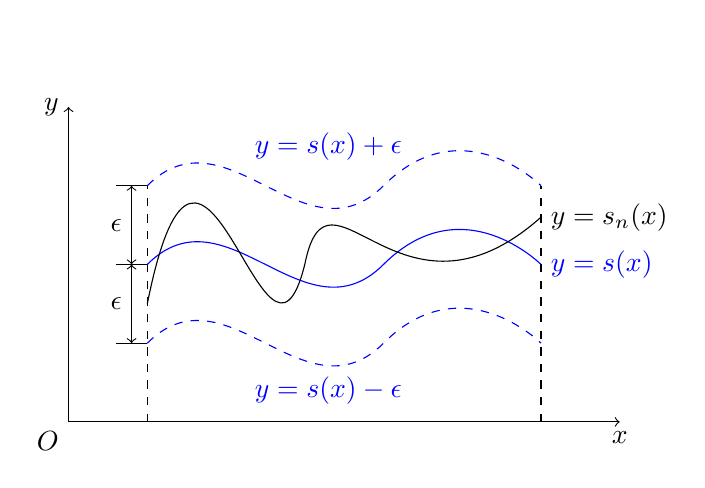
\begin{tikzpicture}
\draw[->](0,0)node[below left]{\(O\)} -- (7,0)node[below]{\(x\)};
\draw[->](0,0) -- (0,4)node[left]{\(y\)};
\draw[dashed](1,0) -- (1,3) (6,0) -- (6,3);
\draw(1,1)--+(-.4,0);
\draw(1,2)--+(-.4,0);
\draw(1,3)--+(-.4,0);
\begin{scope}[<->,xshift=-.2cm]
\draw(1,1) -- (1,2)node[midway,left]{\(\epsilon\)};
\draw(1,2) -- (1,3)node[midway,left]{\(\epsilon\)};
\end{scope}
\begin{scope}[blue]
\draw[dashed] (1,1) .. controls (2,2) and (3,0) .. (4,1) .. controls (5,2) and (6,1) .. (6,1);
\draw[yshift=1cm] (1,1) .. controls (2,2) and (3,0) .. (4,1) .. controls (5,2) and (6,1) .. (6,1)node[right]{\(y = s(x)\)};
\draw[yshift=2cm,dashed] (1,1) .. controls (2,2) and (3,0) .. (4,1) .. controls (5,2) and (6,1) .. (6,1);
\draw(3.3,3.5)node{\(y = s(x) + \epsilon\)};
\draw(3.3,0.4)node{\(y = s(x) - \epsilon\)};
\end{scope}
\draw(1,1.5) .. controls (1.7,5) and (2.5,0) .. (3,2) .. controls (3.3,3.5) and (4.2,1) .. (6,2.6)node[right]{\(y = s_n(x)\)};
\end{tikzpicture}
\caption{函数项级数一致收敛的几何解释}
\label{figure:无穷级数.函数项级数一致收敛的几何解释}
\end{figure}

\begin{example}
研究级数\[
	\frac{1}{x+1} + \left(\frac{1}{x+2}-\frac{1}{x+1}\right)
	+ \dotsb + \left(\frac{1}{x+n}-\frac{1}{x+n-1}\right) + \dotsb
\]在区间\([0,+\infty)\)上的一致收敛性.
\begin{solution}
级数的前\(n\)项和\(s_n(x) = \frac{1}{x+n}\),
因此级数的和\[
	s(x)
	= \lim_{n\to\infty} s_n(x)
	= \lim_{n\to\infty} \frac{1}{x+n}
	= 0
	\quad(0 \leq x < +\infty).
\]
于是,余项的绝对值\[
	\abs{r_n(x)} = \abs{s(x) - s_n(x)}
	= \frac{1}{x+n} \leq \frac{1}{n}
	\quad(0 \leq x < +\infty).
\]
对于\(\forall\epsilon>0\),
取\(N \geq \frac{1}{\epsilon}\),
则当\(n>N\)时,
\(\forall x\in[0,+\infty)\),
有\(\abs{r_n(x)} < \epsilon\).
根据定义,
所给级数在区间\([0,+\infty)\)上一致收敛于\(s(x)\equiv0\).
\end{solution}
\end{example}

\begin{example}
研究级数\[
x + (x^2-x) + \dotsb + (x^n-x^{n-1}) + \dotsb
\]在区间\((0,1)\)上的一致收敛性.
\begin{solution}
这级数在区间\((0,1)\)内处处收敛于和\(s(x)\equiv0\),但并不一致收敛.事实上,这个级数的部分和\(s_n(x) = x^n\).\(\forall n\in\mathbb{N}^+\),取\(x_n = \frac{1}{\sqrt[n]{2}}\),于是\[
s_n(x_n) = x_n^n = \frac{1}{2},
\]但\(s(x_n) = 0\),从而\[
\abs{r_n(x_n)} = \abs{s(x_n) - s_n(x_n)} = \frac{1}{2}.
\]所以,只要取\(\epsilon<\frac{1}{2}\),不论\(n\)多么大,在\((0,1)\)内总存在这样的点\(x_n\),使得\(\abs{r_n(x_n)}>\epsilon\),因此所给级数在\((0,1)\)内不一致收敛.

这表明虽然函数序列\(s_n(x) = x^n\)在\((0,1)\)内处处收敛于\(s(x)\equiv0\),但\(s_n(x)\)在\((0,1)\)内各点处收敛于零的“快慢”程度是不一致的.

可是\(\forall r\in(0,1)\),这级数在\([0,r]\)上一致收敛.这是因为当\(x=0\)时,显然\[
\abs{r_n(x)} = x^n = 0 < \epsilon;
\]当\(0 < x \leq r\)时,要使\(x^n < \epsilon\)(不妨设\(\epsilon < 1\)),只要\(n \ln x < \ln\epsilon\)或\(n > \frac{\ln\epsilon}{\ln x}\);而\(\frac{\ln\epsilon}{\ln x}\)在\((0,r]\)上的最大值为\(\frac{\ln\epsilon}{\ln r}\),故取正整数\(N \geq \frac{\ln\epsilon}{\ln r}\),则当\(n > N\)时,对\([0,r]\)上的一切\(x\)都有\(x^n < \epsilon\).
\end{solution}
\end{example}
上例说明了一致收敛性与所讨论的区间有关.

\subsection{魏尔斯特拉斯判别法}
以上两例都是直接根据定义来判定级数的一致收敛性的,现在介绍一个在实用上较方便的判别法.
\begin{theorem}[魏尔斯特拉斯判别法]\label{theorem:无穷级数.魏尔斯特拉斯判别法}
如果函数项级数\(\sum_{n=1}^\infty u_n(x)\)在区间\(I\)上满足条件\begin{enumerate}
\item \(\abs{u_n(x)} \leq a_n \quad(n=1,2,\dotsc)\);
\item 正项级数\(\sum_{n=1}^\infty a_n\)收敛,
\end{enumerate}
则函数项级数\(\sum_{n=1}^\infty u_n(x)\)在区间\(I\)上一致收敛.
\begin{proof}
由条件2,根据\hyperref[theorem:无穷级数.级数的柯西审敛原理]{柯西审敛原理},
\(\forall\epsilon>0\),\(\exists N \in \mathbb{N}^+\),
使得当\(n > N\)时,\(\forall p \in \mathbb{N}^+\),都有\[
a_{n+1} + a_{n+2} + \dotsb + a_{n+p} < \frac{\epsilon}{2}.
\]由条件1,\(\forall x \in I\),都有\begin{align*}
&\hspace{-20pt}\abs{u_{n+1}(x) + u_{n+2}(x) + \dotsb + u_{n+p}(x)} \\
&\leq \abs{u_{n+1}(x)} + \abs{u_{n+2}(x)} + \dotsb + \abs{u_{n+p}(x)} \\
&\leq a_{n+1} + a_{n+2} + \dotsb + a_{n+p} < \frac{\epsilon}{2},
\end{align*}令\(p\to\infty\),则由上式得\[
\abs{r_n(x)} \leq \frac{\epsilon}{2} < \epsilon.
\]因此函数项级数\(\sum_{n=1}^\infty u_n(x)\)在区间\(I\)上一致收敛.
\end{proof}
\end{theorem}

\begin{example}
证明级数\[
\frac{\sin x}{1^2}
+ \frac{\sin 2^2 x}{2^2}
+ \dotsb
+ \frac{\sin n^2 x}{n^2}
+ \dotsb
\]在区间\((-\infty,+\infty)\)内一致收敛.
\begin{proof}
因为在\((-\infty,+\infty)\)内\[
\abs{\frac{\sin n^2 x}{n^2}} \leq \frac{1}{n^2}
\quad(n=1,2,\dotsc),
\]而\(\sum_{n=1}^\infty \frac{1}{n^2}\)收敛,
故由\hyperref[theorem:无穷级数.魏尔斯特拉斯判别法]{魏尔斯特拉斯判别法},
所给级数在\((-\infty,+\infty)\)内一致收敛.
\end{proof}
\end{example}

\subsection{阿贝尔判别法}
\begin{theorem}[阿贝尔判别法]\label{theorem:无穷级数.阿贝尔判别法}
如果有
\begin{enumerate}
\item 函数项级数\(\sum_{n=1}^\infty a_n(x)\)在区间\(I\)上一致收敛;
\item 函数\(b_n(x)\ (n=1,2,\dotsc)\)都有界,且对任意\(x\)组成一个单调序列;
\end{enumerate}
那么函数项级数\[
	\sum_{n=1}^\infty a_n(x) b_n(x)
\]
在区间\(I\)上一致收敛.
\end{theorem}

\subsection{狄利克雷判别法}
\begin{theorem}[狄利克雷判别法]\label{theorem:无穷级数.狄利克雷判别法}
如果有
\begin{enumerate}
\item 部分和\(\sum_{i=1}^n a_i(x)\)总是有界的;
\item 序列\(\{b_n(x)\}\)对于任意\(x\)都是单调的,
且当\(n\to\infty\)时在区间\(I\)上一致地趋于零;
\end{enumerate}
那么函数项级数\[
	\sum_{n=1}^\infty a_n(x) b_n(x)
\]
在区间\(I\)上一致收敛.
\end{theorem}

\subsection{一致收敛级数的基本性质}
一致收敛级数有如下基本性质.
\begin{property}\label{theorem:无穷级数.一致收敛级数的基本性质1}
\def\su{\sum_{n=1}^\infty u_n(x)}
如果级数\(\su\)的各项\(u_n(x)\)在区间\([a,b]\)上都连续,且\(\su\)在区间\([a,b]\)上一致收敛于\(s(x)\),则\(s(x)\)在\([a,b]\)上也连续.
\begin{proof}
设\(x_0,x\)是\([a,b]\)上任意两点.由等式\[
s(x) = s_n(x) + r_n(x),
\qquad
s(x_0) = s_n(x_0) + r_n(x_0)
\]得\begin{align*}
\abs{s(x) - s_(x_0)}
&= \abs{s_n(x) - s_n(x_0) + r_n(x) - r_n(x_0)} \\
&\leq \abs{s_n(x) - s_n(x_0)} + \abs{r_n(x)} + \abs{r_n(x_0)}.
\tag1
\end{align*}
因为级数\(\su\)一致收敛于\(s(x)\),所以\(\forall\epsilon>0\),必有正整数\(N = N(\epsilon)\),使得当\(n>N\)时,\(\forall x \in [a,b]\),都有\[
\abs{r_n(x)} < \frac{\epsilon}{3}.
\eqno(2)
\]当然,也有\(\abs{r_n(x_0)} < \frac{\epsilon}{3}\).选定满足大于\(N\)的\(n\)之后,\(s_n(x)\)是有限项连续函数之和,故\(s_n(x)\)在点\(x_0\)连续,从而必有一个\(\delta > 0\)存在,当\(\abs{x - x_0} < \delta\)时,总有\[
\abs{s_n(x) - s_n(x_0)} < \frac{\epsilon}{3}.
\eqno(3)
\]由(1)、(2)、(3)式可见,对任给\(\epsilon>0\),必有\(\delta > 0\),当\(\abs{x - x_0} < \delta\)时,有\[
\abs{s(x) - s(x_0)} < \epsilon.
\]所以\(s(x)\)在点\(x_0\)连续,而\(x_0\)在\([a,b]\)上是任意的,因此\(s(x)\)在\([a,b]\)上连续.
\end{proof}
\end{property}

\begin{property}\label{theorem:无穷级数.一致收敛级数的基本性质2}
若函数项级数\(\sum_{n=1}^\infty u_n(x)\)在区间\(I\)上内闭一致收敛,且\[
\lim_{x \to a} u_n(x) = A_n
\quad(n=1,2,\dotsc),
\]
则级数\(\sum_{n=1}^\infty A_n\)收敛,且\[
\lim_{x \to a} \left\{
	\sum_{n=1}^\infty u_n(x)
\right\}
= \sum_{n=1}^\infty \left\{
	\vphantom{\sum_{n=1}^\infty }
	\lim_{x \to a} u_n(x)
\right\}.
\]
\end{property}

\begin{property}\label{theorem:无穷级数.一致收敛级数的基本性质3}
如果级数\(\sum_{n=1}^\infty u_n(x)\)的各项\(u_n(x)\)在区间\([a,b]\)上都连续,
且\(\sum_{n=1}^\infty u_n(x)\)在区间\([a,b]\)上一致收敛于\(s(x)\),
则级数\(\sum_{n=1}^\infty u_n(x)\)在\([a,b]\)上可以逐项积分,
即\[
	\int_{x_0}^x s(x) \dd{x}
	= \sum_{n=1}^\infty \int_{x_0}^x u_n(x) \dd{x},
\]
其中\(a \leq x_0 < x \leq b\),并且上式右端的级数在\([a,b]\)上也一致收敛.
\begin{proof}
因为级数\(\sum_{n=1}^\infty u_n(x)\)在\([a,b]\)上一致收敛,
由\cref{theorem:无穷级数.一致收敛级数的基本性质1},
\(s(x)\)和\(r_n(x)\)都在\([a,b]\)上连续,
所以积分\(\int_{x_0}^x s(x) \dd{x}\)和\(\int_{x_0}^x r_n(x) \dd{x}\)存在,
从而\[
	\abs{\int_{x_0}^x s(x) \dd{x} - \int_{x_0}^x s_n(x) \dd{x}}
	= \abs{\int_{x_0}^x r_n(x) \dd{x}}
	\leq \int_{x_0}^x \abs{r_n(x)} \dd{x}.
\]
又由级数的一致收敛性,
\(\forall\epsilon>0\),
\(\exists N = N(\epsilon) \in \mathbb{N}^+\),
使得当\(n > N\)时,
\(\forall x \in [a,b]\),
都有\[
	\abs{r_n(x)} < \frac{\epsilon}{b-a}.
\]
于是,当\(n > N\)时,有\[
	\abs{\int_{x_0}^x s(x) \dd{x} - \int_{x_0}^x s_n(x) \dd{x}}
	\leq \int_{x_0}^x \abs{r_n(x)} \dd{x}
	< \frac{\epsilon}{b-a} \cdot (x-x_0)
	\leq \epsilon.
\]
根据极限的定义,有\[
	\int_{x_0}^x s(x) \dd{x}
	= \lim_{n\to\infty} \int_{x_0}^x s_n(x) \dd{x}
	= \lim_{n\to\infty} \sum_{i=1}^n \int_{x_0}^x u_i(x) \dd{x}
	= \sum_{n=1}^\infty \int_{x_0}^x u_n(x) \dd{x}.
\]
由于\(N\)只依赖于\(\epsilon\)而与\(x_0,x\)无关,
所以级数\(\sum_{n=1}^\infty \int_{x_0}^x u_n(x) \dd{x}\)在\([a,b]\)上一致收敛.
\end{proof}
\end{property}

\begin{property}\label{theorem:无穷级数.一致收敛级数的基本性质4}
如果级数\(\sum_{n=1}^\infty u_n(x)\)的各项\(u_n(x)\)都具有连续导数\(u'_n(x)\),
且\(\sum_{n=1}^\infty u_n(x)\)在区间\([a,b]\)上收敛于和\(s(x)\),
它并且级数\(\sum_{n=1}^\infty u'_n(x)\)在\([a,b]\)上一致收敛,
则级数\(\sum_{n=1}^\infty u_n(x)\)在区间\([a,b]\)上也一致收敛,且可逐项求导,
即\[
	s'(x) = \sum_{n=1}^\infty u'_n(x).
\]
\begin{proof}
由于\(\sum_{n=1}^\infty u'_n(x)\)在\([a,b]\)上一致收敛,设其和为\(v(x)\),即\[
	\sum_{n=1}^\infty u'_n(x) = v(x).
\]
根据\cref{theorem:无穷级数.一致收敛级数的基本性质1} 知,
\(v(x)\)在\([a,b]\)上连续.
再根据\cref{theorem:无穷级数.一致收敛级数的基本性质3},
级数\(\sum_{n=1}^\infty u'_n(x)\)可逐项积分,故\[
	\int_{x_0}^x v(x) \dd{x}
	= \sum_{n=1}^\infty \int_{x_0}^x u'_n(x) \dd{x}
	= \sum_{n=1}^\infty [u_n(x) - u_n(x_0)],
\]
而\(\sum_{n=1}^\infty u_n(x) = s(x)\),
\(\sum_{n=1}^\infty u_n(x_0) = s(x_0)\),
故\[
	\sum_{n=1}^\infty [u_n(x) - u_n(x_0)]
	= s(x) - s(x_0),
\]
从而有\[
	\int_{x_0}^x v(x) \dd{x} = s(x) - s(x_0),
\]
其中\(a \leq x_0 < x \leq b\).
上式两端求导,即得关系式\[
	v(x) = s'(x).
\]

根据\cref{theorem:无穷级数.一致收敛级数的基本性质3},
级数\(\sum_{n=1}^\infty \int_{x_0}^x u'_n(x) \dd{x}\)在\([a,b]\)上一致收敛,而\[
	\sum_{n=1}^\infty \int_{x_0}^x u'_n(x) \dd{x}
	= \sum_{n=1}^\infty u_n(x)
		- \sum_{n=1}^\infty u_n(x_0),
\]所以\[
	\sum_{n=1}^\infty u_n(x)
	= \sum_{n=1}^\infty \int_{x_0}^x u'_n(x) \dd{x}
	+ \sum_{n=1}^\infty u_n(x_0).
\]也就是说,级数\(\sum_{n=1}^\infty u_n(x)\)在\([a,b]\)上一致收敛.
\end{proof}
\end{property}
